% !TEX root = ../thesis.tex
% !TEX spellcheck = en-US

\clearpage

\section{Exploration}
\label{sec:Exploration}

The first part of this thesis project was dedicated to the exploration of the problem space. Driven by the \nameref{sub:Research Scope and Objectives} (see Section~\ref{sub:Research Scope and Objectives}) the goal of this phase was twofold: At once to find an approachable yet challenging research problem in the context of data from a recruitment platform and secondly to simultaneously evaluate the potential to create business value through an enhanced user experience or new use cases for the service \gls{Oikotie Tyopaikat}. The exploration is divided into a discovery phase where the problem scope diverges and a definition phase where it converges as described in Section~\ref{sub:Methodological Approach}. In the following sections we will look at the process and results of these phases in detail.

\subsection{Discovery Phase: Exploring the Problem Scope}
\label{Discovery Phase: Exploring the Problem Scope}

During the discovery phase the problem space was first opened up through exploration of user needs and initial field research to better understand the problem context. Additionally literature research and benchmarking of approaches helped getting a picture of related scientific work. It should be noted though that in-depth user research was kept at an absolute minimum due to time constraints and the scientific focus of this thesis.

Initially a set of interviews with stakeholders from Product Management to Marketing and Engineering working on the product as well as potential users helped obtaining a good understanding about the service offerings of a recruitment platform and the current trends in the industry. Exploring the various data that the platform generates, an important learning was that large parts of the data are in form of written language and much of it in a more or less unstructured way.

Exploration was therefore focused on language related problems. Literature research revealed a strong interest from the research community in tasks related language modeling using neural networks and related connectionist approaches that have gained traction recently through the latest advances of \gls{Deep Learning}. Several methods were then tested as quick prototypes. A side-effect was the (re-)realization that real data is often noisy and inconsistent. In addition ideas for focusing the problem search were evaluated, ranging from practical ideas such as predicting trends in the job market to wilder ones such as digitalizing the complete Sanoma archive to analyze how written language evolves over time in order to predict when a text was written or to identify trending terms or writing styles from a certain period of time.

Through further experimentation, research and discussions, the problem of utilizing the implicit knowledge in the text body of job listings was deemed a good fit for further focus. It was both an interesting and challenging research problem and could potentially be of practical use, e.g.\ when identifying the requirements for a job inside this text. This decision set the course for the definition phase to begin with increased focus on narrowing explored set of problems to a single problem definition.

\subsection{Definition Phase: Framing the Problem}
\label{sub:Definition Phase: Framing the Problem}

The definition phase of the design process is characterized by explorative convergence of the problem space through iterative reframing and refinement of the problem definition, hand in hand with further experimentation and learning within the new scope. In the case of this research project it is marked by three main decision points where the problem definition was reformulated.
These three iterations of converging towards a final problem definition are described next in terms of rationale for the chosen direction, the experimental approach to learn within this new scope and the results and learnings obtained.

\subsubsection{Inferring Structure of Job Advertisements}
\label{subs:Inferring Structure in Job Advertisements}

\paragraph{Rationale}
\label{par:Rationale (Inferring Structure of Job Advertisements)}

During the discovery phase it became apparent that a there is large amounts of unstructured and implicit knowledge in the data of job advertisements. Specifically large portions of the data are natural language in relatively free form. One example for this which also makes up a significant amount of data is the text body of each job advertisement. This part, just like the content of a job listing in print media, contains all the information about a job position that a company wants to communicate to a potential applicant.

The contained information can be useful to provide better services, e.g.\ by inferring requirements for a job from the text in order to show more relevant listings to the user. Another potential application of \gls{Machine Learning} to this data is to predict popularity within certain target audiences for job advertisements, for instance to help recruiters design better job listings. In many cases it is useful for these applications to first better have a better representation of the structure and content of the job ad. Thus learning the structure of job advertisements was set as a subject of further study.

\paragraph{Experimental Approach}
\label{par:Experimental Approach and Metrics}

To learn how humans interpret structure and content of job ads and what they consider a good structural representation of the information contained a set of experiments was carried out. Five participants from various professional background were asked to highlight sections of the text in a job advertisement and to label these sections by describing what the section is about. Afterwards they were asked to restructure the job ad into a bullet-point list based on these highlighted sections.

No specific metrics were used as this experiment was purely explorative to gain a basic understanding how terms like \emph{structure} and \emph{content} or \emph{topics} are interpreted and applied given the job listing samples. Each participant was provided with a \gls{Google Docs} document including one random job advertisement in English and the tasks that were formulated as follows:

\blockquote{Cheers for helping out with this little experiment for my thesis! My aim here is to find out how people would structure job ads to help find the relevant information faster.

You'll work with the job advertisement below. Your task is the following:
\begin{enumerate}
  \item First tag the job advertisement below into parts. Mark sections of it and use a word or two to categorize this section using the comment tool. You can tag the ad into sections however you want and even make the sections overlap. The goal here is to tag the content of the job ad that you think belongs to different categories, properties or topics. To tag the text, use the comment tool like this: ``We're looking for a Quality Buzzword Engineer.''
  \item Now fill the bullet-point list in the last section of this document with the tagged sections/categories/topics you found. It should roughly contain the same information as the ad but in a structured way using your tags. You can use sub-points categories if you want.
\end{enumerate}
In total try to spend no more than 30 minutes on this. Don't worry about it too much, the key is to just do it how it makes sense to you.}

A full example of this task as it was provided for the participants can be found in the Appendix in Section~\ref{sub:Understanding How Humans Structure Text}.

\paragraph{Results}
\label{par:Results (Inferring Structure of Job Advertisements)}

After initially expressing difficulties with the open and ambiguous task participants were provided with help by providing analogous examples (e.g.\ to label the description of a car, which parts describe the components while others talk about the owner etc.). While this helped it was still perceived as a very difficult task as it leaves lots of room for interpretation.
The outcomes were quite various, especially along the following spectra:

\begin{itemize}
  \item Generality versus specificity: A section about the language requirements was labelled as \emph{Requirements} by one participant and a similar section as \emph{language requirements}
  \item Content versus structure: A heading was described in one instance as \emph{Job description} and a very similar one by another participant as \emph{Job description section indicator}
  \item Objectivity versus judgement: Some sections were judged by their content, e.g.\ as \emph{Empty words}
\end{itemize}

Also some participants built a nested structure in the second part of the task while others formulated rather wide areas to group the information in a flat list of topics.

\paragraph{Learnings and Conclusions}
\label{par:Learnings and Conclusions (Inferring Structure of Job Advertisements)}

One meaningful learning was that also explorative experiments need to be constrained and well-defined as posing the question so openly lead to great difficulties understanding and performing it and to diffuse outcomes. However it gave some initial insight in possible ways to capture and structure this type of texts in job advertisements and sparked discussions for the following research. Thus the problem of structuring job advertisements was set up for refinement through an experiment of larger scale.

\subsubsection{Supervised Multi-label Paragraph Classification}
\label{subs:Supervised Multi-label Paragraph Classification}

\paragraph{Rationale}
\label{par:Rationale (Multi-label Paragraph Classification)}

Following the learnings about how participants interpreted the structure of job listings the problem was divided into three sub-problems:

\begin{enumerate}
  \item Finding sections of text that form semantic units
  \item Identify a label that communicates the function or meaning of these units
  \item Infer a hierarchy over the labels and therefore also over the structure of the sections
\end{enumerate}

As each of these problems is a challenge of its own the focus was laid on finding the labels of sections while fixing the sections to be paragraphs and ignoring the possibility of a hierarchy of the labels. It seemed a valuable outcome to be able to classify text segments and feasible to evaluate.
This implied another important decision in terms of problem structure: The task was set up to be a \gls{Supervised Learning} problem. As mentioned in~\nameref{sub:Related work} (Section~\ref{sub:Related work}), \gls{Topic Modeling} and related fields are very relevant to this kind of research problem which are \gls{Unsupervised Learning} approaches.
While certainly a possibility to frame the problem in that way, the rationale behind the choice of a supervised problem setting was that it makes the task much easier to systematically evaluate as expected outcomes are given. Further it was of potential interest in the context of the service that specific topics could identified that are known to be existent in the data as well as possible which seemingly could lead to more accurate results when taking a supervised approach.

Based on these constraints a new experiment was set up where paragraphs were labelled by participants through a purpose-built web interface. The the aim was to collect a larger sample of data that would be better quantifiable, less biased and more representative through a higher number of participants, and to use this data for deepening the understanding of the problem and to evaluate the feasibility of tackling it with first proof-of-concept prototype experiments.

\paragraph{Crowd-sourced Data Collection}
\label{par:Crowd-sourced Data Collection}

To collect the data a tool was build, consisting of a \gls{Node.js} server using \gls{MongoDB} as a database and communicating via a \acrshort{JSON} \acrshort{REST} \acrshort{API} with a simple website front-end using the \gls{Mustache} template engine.
The used data were job advertisements from the \gls{Oikotie Tyopaikat} job recruitment platform. The full dataset consists of 118.780 job ads published between September 01, 2012 and December 01, 2015. Using the tool \gls{langdetect}, 9928 of these job advertisements were identified to be written in English language. This corresponds to approximately 8.4\% of the dataset, as opposed 75\% of postings that are written in Finnish. These English job listings were then split into paragraphs with a simple rule-based approach that can be seen in the software package (see Appendix, Section~\ref{sub:thesis-tagger: A Tool for Tagging Chunked Job Ads} for a description and a link to the source code on \gls{GitHub})\footnote{see \url{https://github.com/cle-ment/thesis-tagger/blob/master/pre-processing.ipynb} for the specific preprocessing procedure of the job ad data.}.

The exact task given to the participants was: \emph{``Describe what each section is about by adding one or more tags/keywords to it''}. Participants were shown a job ad that was split into paragraphs and besides each paragraph was a text field to enter one or more tags as Figure~\ref{fig:thesis-tagger interface} shows.

\begin{figure}[h]
  \centering
  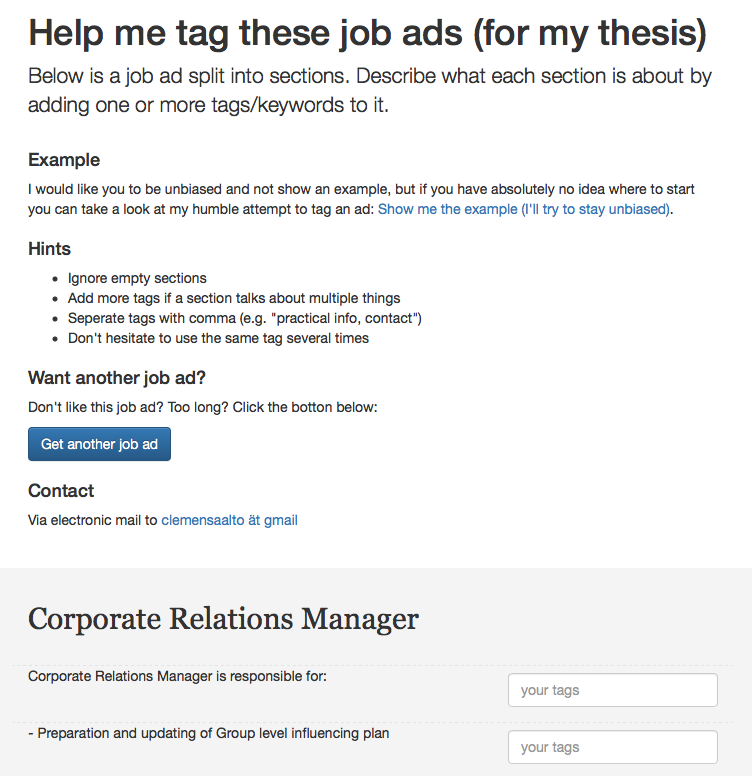
\includegraphics[width=0.9\textwidth]{img/thesis-tagger-interface.png}
  \caption{Screen capture of the interface of the tagging tool}
\label{fig:thesis-tagger interface}
\end{figure}

In a first step the tool was only shown to 3 participants to get immediate feedback if the user interface had flaws and whether the task was understood. Based on this feedback the tool was improved by providing an example for the participants and then tested with a slightly larger group of 12 persons. After correcting a few minor details in the user interface a public link was then shared via social media and other chNNels to as many people as possible. A few days later the tool was then also shared internally within Sanoma where it was set up as a competition to tag the most possible job ads, increasing participation significantly. In total 91 job ads were tagged, resulting in 379 tagged text sections and 358 tags.

\paragraph{Initial Experiments}
\label{par:Initial Experiments}

To test whether automatic prediction of the obtained labels for paragraphs was possible a small prototype was build. Since every paragraph was potentially assigned multiple labels this first experiment was framed as a \gls{Multi-Label Classification} problem where the absence or presence of each label is predicted for a paragraph. For classification a TF.IDF weighted Unigram model was applied that uses the frequencies of words associated with a label to create mappings for these labels in a common vector space. Using this vector space we can then apply various classification algorithms with the assumption that closeness of labelled data in the vector space translates to similarity of the associated objects in the real world domain (see Section~\ref{subs:N-gram Models (Methods)} for details on these types of models).

Using a \gls{kNN} approach the $k$ most probable labels were predicted and was called a success if the true labels intersected with the predicted ones. Using 10-fold \gls{Cross-Validation} this lead to a success rate of 0.32 for $k=5$, 0.24 for $k=3$ and 0.1 for $k=1$, while random predictions constantly performed a success rate of 0. This can be regarded as rather poor performance if the task is to predict the most relevant label. However it has to be considering that the task for assigning the labels was very loosely defined and the sample of data was rather small, both leading to extremely sparse data. Most labels were only used once or twice so that their data pool was only one or two paragraphs of text. While there was much room for improvement, this experiment also showed that even with sparse data learning structure with regards to the problem is possible.

\paragraph{Structuring the Data}
\label{par:Structuring the Data}

Inspection of the collected labels showed that many labels correlated, being synonyms, different versions of spelling the same term or were simply in terms of meaning. To capture this structure and try to disambiguate labels the data was clustered using two different approaches, once algorithmically and once manually. First algorithmic clustering was carried out with using \gls{Lloyds Algorithm} for \gls{K-means Clustering}. Effectiveness of the clustering was measured using the \gls{Silhouette Score} while testing different numbers of clusters $k$. The Silhouette Score did not indicate a clear minimum at any point. Further visualization of the resulting structure showed seemingly arbitrary changes in the assignment to clusters varying the number of clusters and thus no reliable grouping could be extracted.
Given the sparsity of the data the high variance of the outcomes were not unexpected however.

As a next attempt the data was sorted manually into a hierarchy. The grouping of labels was first done with a manual ``Chinese Restaurant Process'' \todo{glossary?}, i.e.\ the first label defined the first group and each successive label in the list was either added to one of the existing groups due to similarity or a new group was created.
From this analysis different types of groups emerged, some of which overlapped in meaning. Thus as a second approach a top down process helped identify groups in a similar domain of meaning and which were largely complimentary and non-overlapping.
Figure~\ref{fig:job-listing-structure} shows a high-level result of this grouping. The data was then clustered into done the top-level nodes in Figure~\ref{fig:job-listing-structure}: \emph{Summary: Short introduction}, \emph{Person specification (Who you are)}, \emph{Job specification (What you give)}, \emph{Company (Who we are)}, \emph{Next steps} and \emph{Other}. The full results the manual top-down clustering can be seen in the Appendix, Section~\ref{sub:Collected Labels in Paragraph Experiment} in \acrshort{JSON} format.

\begin{figure}[h]
  \centering
  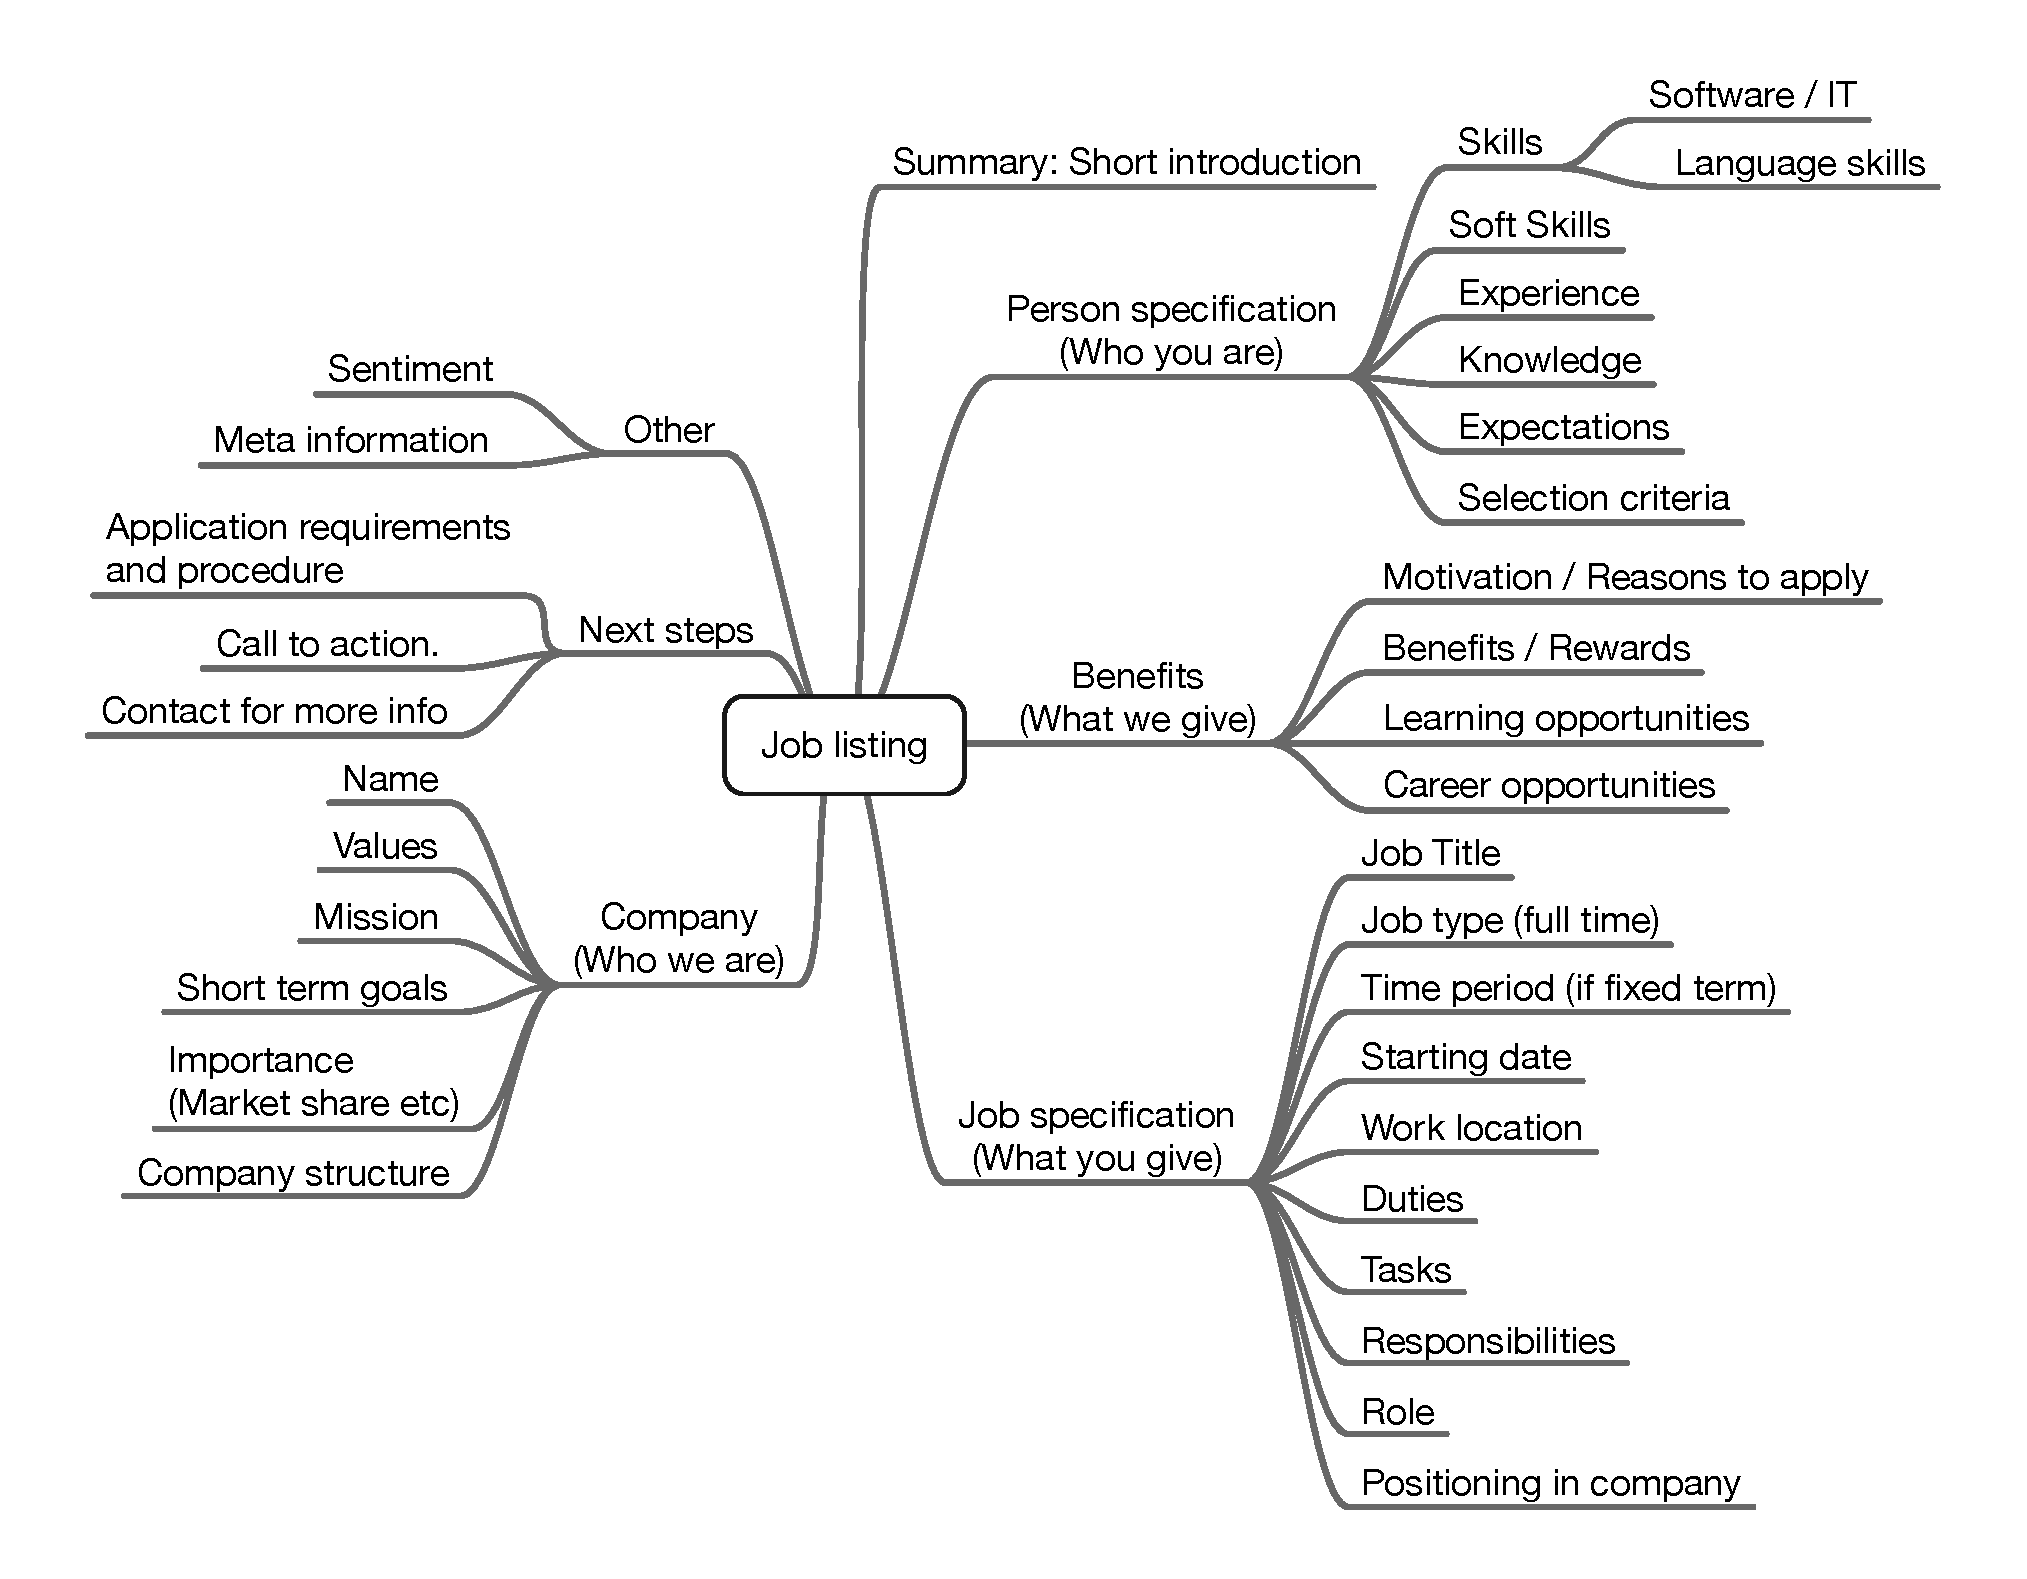
\includegraphics[width=\textwidth]{img/job-listing-structure.pdf}
  \caption{Structure of job listings inferred from the labels given by participants.}
\label{fig:job-listing-structure}
\end{figure}

\paragraph{Classification Experiments on Clustered Data}
\label{par:Classification Experiments on Clustered Data (Multi-label Paragraph Classification)}

After clustering the data further classification experiments were carried out, this time framed as a \gls{Multi-Class Classification} problem, i.e.\ assuming that classes are distinct. A wider array of classifiers was used on the data, including most of the algorithms described in Section~\ref{sub:Methods For Classification With Vector Space Models}: Logistic Regression, Decision Tree, Naive Bayes, SVM, kNN, Random Forest and a Neural Network with a single hidden layer. Performance was measured in $F1$ Score since at this point it was easier to use and while biased has similar properties to \gls{MCC} (see Section~\ref{sub:Evaluation Metrics} for more information on the different performance metrics). All methods performed considerably well with an F1 test score of 0.55 - 0.60 (except \gls{kNN} which only achieved 0.30). The label \emph{Summary: Short introduction} received on average 10\% lower scores across all classifiers.

\paragraph{Learnings and Conclusions}
\label{par:Learnings and Conclusions (Multi-label Paragraph Classification)}

The results using the clustered data gave confirmation to continue refining the problem towards this direction. The experiments showed that it is possible to learn enough structure even with a sparse and noisy dataset at hand to predict the topics of paragraphs to a certain extent. Further it showed that the grouping that was imposed manually based on exploring the collected data lead to separability meaning that the supervised setting with explicit labels is a valid choice to model the problem of identifying structure in job advertisements.

As mentioned above, an exception with regards to separability was the class \emph{Summary: Short introduction} whose data points were often classified as belonging to other classes. A closer look at the actual text in this category revealed that this behavior was not an inability to pick up the characteristics of this class by the algorithm but in fact most examples could indeed have been easily assigned to one of the other classes. This observation also lead to the realization that this class is a grouping based on the position within the job advertisement while all other class labels express the content or topics of the paragraph. Thus the label was removed, leading to the six labels which were used in the next stage.

Another important observation when exploring the data was that often paragraphs could be separated further with regards to the six labels chosen. Thus the separation of text into paragraphs was too coarse-grained. This led to the decision to split the data on sentence-level in the next phase.

\subsubsection{Multi-class Sentence Classification}
\label{subs:Multi-class Sentence Classification}

\paragraph{Rationale}
\label{par:Rationale}

Towards the end of the definition phase --- and with it the exploration phase of the project --- the aim was to converge towards a final problem definition that would be the focus of research for the rest of the project where the best solution approach would be evaluated. The paragraph classification experiments and their refinements proved a promising direction. For exploration the problem was previously left open to interpretation on purpose, it now needed to be reframed as a well-defined, constrained and meaningful problem definition. This was to ensure that the problem solved was relevant and modeled the problem domain in a realistic way. Further conventions from related work with regards to the problem formalization were adapted to show the relation and possible differences and put the results into perspective from a academic point of view.

With the learnings from the previous phase the problem was formulated as \emph{sentence-level} \gls{Multi-Class Classification}. The classes used were \emph{benefits, candidate, company, job, nextsteps, other}  and were assumed to be distinct. The semantics behind these classes came from the previous experiments and are explained in Section~\ref{subs:Dataset: Labelled Sentences from Job Advertisements} in more detail.

\paragraph{Crowd-sourced Data Collection via Crowdflower}
\label{par:Crowd-sourced Data Collection via Crowdflower}

In order to evaluate approaches to the problem task a labelled dataset of sentences was needed. For this purpose the \gls{Mikrotasking} service \gls{CrowdFlower} was chosen over its competitor platform \gls{Amazon Mechanical Turk} due to the simple practical reason that the latter required the paying party to be an american resident.
The source of data was the same dataset as in the previous experiments --- a dataset of English job advertisements from the service \gls{Oikotie Tyopaikat}. Here 400 job english listings were selected at random and converted into a set of 10670 english sentences using the \emph{Punkt Sentence Tokenizer}\footnote{See \url{http://www.nltk.org/api/nltk.tokenize.html\#module-nltk.tokenize.punkt}} of the \gls{NLTK}. Afterwards the sentences were converted from HTML into raw text using the \gls{Beautiful Soup} package.

The task setup was improved over several rounds of pilot testing with a few hundred rows of data. The main learnings were in terms of posing fair test questions, i.e.\ questions to test participants on pre-labelled data, and further in the formulation of instructions to make the task easily comprehensible for the participants. For the final data collection each sentence was labeled thrice by different participants. This was done to assess the confidence of results in terms agreement between participants.

confirmed that the task was well-defined and solvable for humans to a good degree

The resulting dataset contained a total of 9948 sentences (93.23\% of the data) with an inter-subject agreement of over 60\%, meaning that at least two of three participants agreed on the label. Further only 4.74\% of the sentences were labelled as \emph{other}. Figure~\ref{fig:sentence-data-judgements} shows the distribution of the confidence regarding the labels.

\begin{figure}[h]
 % From http://localhost:8888/notebooks/thesis/experiments/vector-space-models/Vector%20Space%20Models.ipynb#Setup
    \centering
    \begin{subfigure}[b]{0.46\textwidth}
        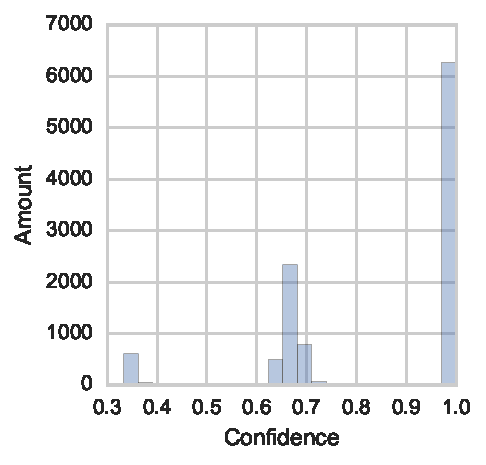
\includegraphics[width=\textwidth]{img/sentence-data-judgement-confidence.pdf}
        \caption{Confidence}
\label{fig:sentence-data-judgement-confidence}
    \end{subfigure}
~%add desired spacing between images, e. g. ~, \quad, \qquad, \hfill etc.
    %(or a blank line to force the subfigure onto a new line)
    \begin{subfigure}[b]{0.43\textwidth}
        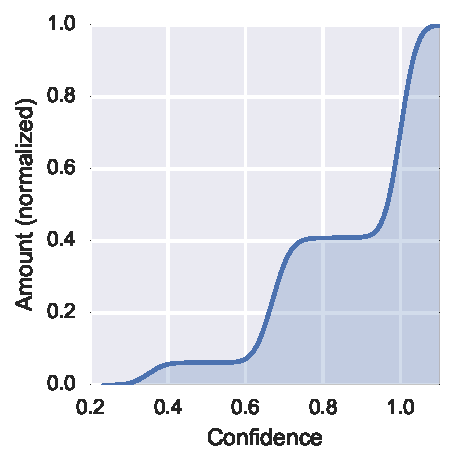
\includegraphics[width=\textwidth]{img/sentence-data-judgement-confidence-cumulative.pdf}
        \caption{Cumulative Confidence}
\label{fig:sentence-data-judgement-confidence-cumulative}
    \end{subfigure}
    \caption{Amount of label judgements versus label confidence based on agreement}
\label{fig:sentence-data-judgements}
\end{figure}

\paragraph{First Experiments and Conclusions}
\label{par:First Experiments and Conclusions}

To confirm that the dataset was a good representation of the problem and offered opportunity for learning algorithms to predict on unseen data a series of fast experiments was carried out.
For this purpose a small set of algorithms was used including Logistic Regression and Naive Bayes using N-grams (see Section~\ref{sub:Vector Space Models}). Results showed a \gls{MCC} test score of over 0.6 and F1 Scores of around over 0.65 which was. This was an improvement compared to the multi-class setup for paragraph prediction in the previous section (0.55 - 0.60 F1 score).
It is important to keep in mind that this is not a fair comparison as the dataset was now consisted of sentences instead of paragraphs and was much larger.
Nevertheless these first Experiments and Results along with the fact that only a small portion of data was labelled as \emph{other} gave were a confirmation that a well-defined scope and setting for further research was now found, finalizing the problem definition phase. Furthermore, as discussed in the discovery phase in Section~\ref{Discovery Phase: Exploring the Problem Scope} there was potential for several application business use cases which are beyond the scope of this thesis, ensuring that the research objectives could be met.
